\documentclass{article}
% Chinese
% \documentclass[UTF8, nofonts, mathptmx, 12pt, onecolumn]{article}
% \usepackage{xeCJK}
% \setCJKmainfont{SimSun}
\usepackage{amsmath}
\usepackage{amsfonts}
\usepackage{amssymb}
\usepackage{wasysym}
% \usepackage{ctex}
\usepackage{graphicx}
\usepackage{float}
\usepackage{geometry}
\geometry{a4paper,scale=0.8}
\usepackage{caption}
\usepackage{subcaption}
% \newcommand{\oiint}{\mathop{{\int\!\!\!\!\!\int}\mkern-21mu \bigcirc} {}}
\newcommand*{\dif}{\mathop{}\!\mathrm{d}}
\newcommand*{\md}{\mathop{}\!\mathrm{d}}
\newcommand*{\me}{\mathrm{e}}

\usepackage{parskip}
\setlength{\parindent}{0cm}

\usepackage{bm}
\let\Oldmathbf\mathbf
\renewcommand{\mathbf}[1]{\boldsymbol{\Oldmathbf{#1}}}
\let\eqnarray\align

\renewcommand*{\arraystretch}{2}
\usepackage{units}
\renewcommand{\frac}{\nicefrac}

\usepackage{cellspace}
\setlength{\cellspacetoplimit}{5pt}
\setlength{\cellspacebottomlimit}{5pt}

\author{Xiping Hu}
\usepackage{authblk}
\author{Xiping Hu}
\affil{https://hxp.plus/}
\title{Homework for Chapter 5}

\begin{document}
\maketitle

\begin{figure}[H]
  \centering
  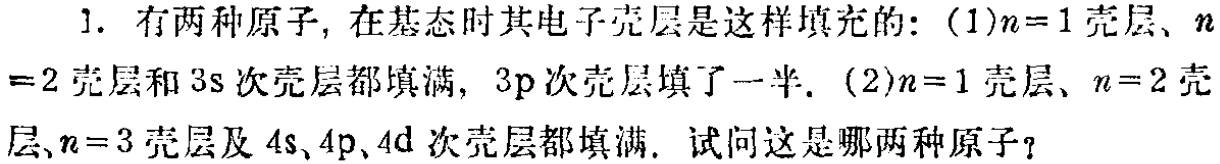
\includegraphics[width=\linewidth]{figures/Problem1}
  \label{fig:}
\end{figure}

The maximum number of electrons a shell may have is shown below

\begin{table*}[h]
  \centering
  \begin{tabular}{|Sc||Sc|Sc|Sc|Sc||Sc|}
    \hline
    n & s & p & d & f & Total \\
    \hline
    1 & 2 & 0 & 0 & 0 & 2 \\
    \hline
    2 & 2 & 6 & 0 & 0 & 8 \\
    \hline
    3 & 2 & 6 & 10 & 0 & 18 \\
    \hline
    4 & 2 & 6 & 10 & 14 & 32 \\
    \hline
  \end{tabular}
\end{table*}

So that the first atom has 15 electrons, which is Phosphor, the second one has 46 electrons, named in Palladium.

\begin{figure}[H]
  \centering
  
\includegraphics[width=\linewidth]{figures/Problem4}
  \label{fig:}
\end{figure}

Answers: (1) $2$ (2) $2l + 1$ (3) $2n^2$

\begin{figure}[H]
  \centering
  
\includegraphics[width=\linewidth]{figures/Problem5}
  \label{fig:}
\end{figure}

From this graph below we can know that

\begin{itemize}
\item for Potassium at $Z = 19$, the spectroscopic term $T$ of 3d is lesser than 4s.
\item for Scandium at $Z = 21$, the spectroscopic term $T$ of 3d is greater than 4s.
\end{itemize}

\begin{figure}[H]
  \centering
  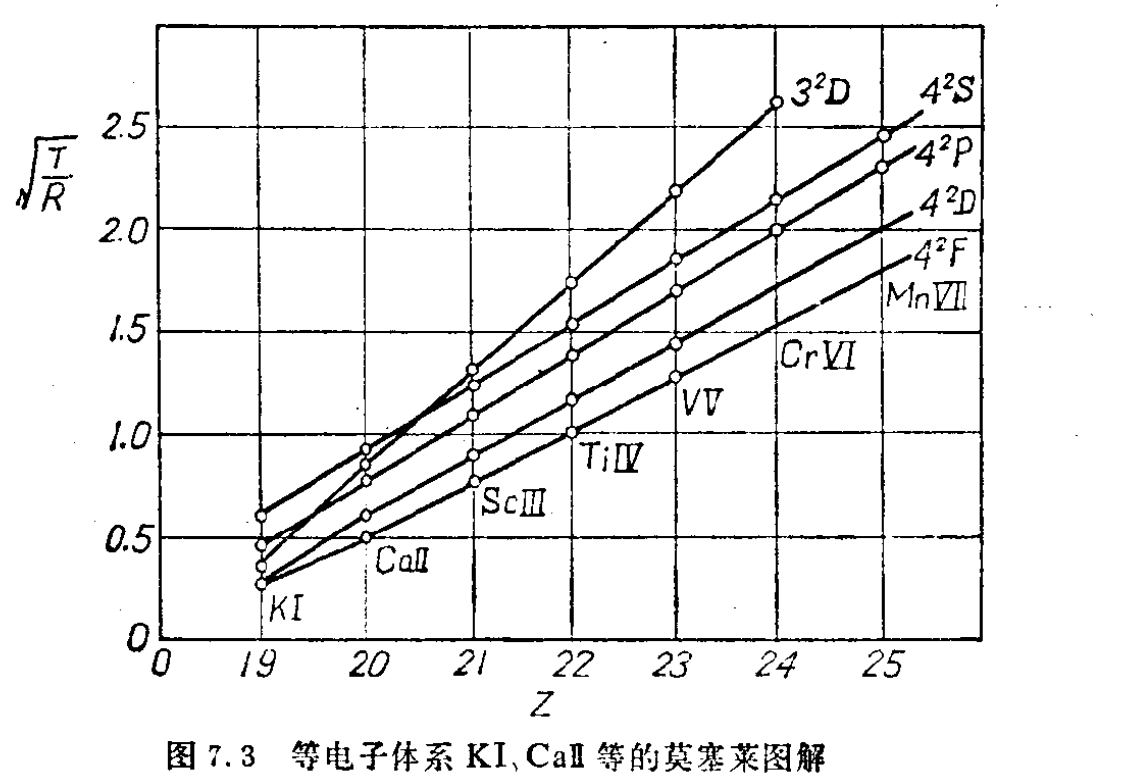
\includegraphics[width=\linewidth]{figures/Problem51}
  \label{fig:}
\end{figure}

Since $E = - h c T$, the energy of electrons is inversely promotional to its spectroscopic term. So that

\begin{itemize}
\item for Potassium at $Z = 19$, the energy $E$ of 3d is greater than 4s.
\item for Scandium at $Z = 21$, the energy $E$ of 3d is lesser than 4s.
\end{itemize}

This is the reason why electrons tend to fill the 4s layer of Potassium and tend to fill the 3d layer of Scandium.

\end{document}